\documentclass[11pt]{article}

\usepackage{amssymb}
\usepackage{amsmath}
\usepackage{multicol}
\usepackage{graphicx}
\usepackage{chngpage}
\usepackage{fancyhdr}
\usepackage[braket, qm]{qcircuit}
\usepackage[font=small,labelfont=bf]{caption}
\usepackage[hidelinks]{hyperref}

\renewcommand*{\arraystretch}{1.15}

\pagestyle{fancy}
\lhead{}

\title{\textbf{Introduction to Quantum Computing}}
\author{Steven Oud \\ \emph{soud@pm.me}}
\begin{document}

\vfill
\maketitle

\tableofcontents

\newpage

\section{Fundementals: A One-Qubit World}
\subsection{What Is Quantum Computing?}
``\emph{Quantum computers are machines that rely on characteristically quantum phenomena, such as quantum interference and quantum entanglement, in order to perform computation.}" - Artur Ekert

\subsection{What Is Quantum Computing Not?}
``\emph{It is tempting to say that a quantum computer is one whose operation is governed by the laws of quantum mechanics. But since the laws of quantum mechanics govern the behavior of all physical phenomena, this temptation must be resisted. Your laptop operates under the laws of quantum mechanics, but it is not a quantum computer.}" - N. David Mermin

\subsection{The Qubit}
A qubit - like a classical bit - has a \emph{state}. In classical bits, this is 0 or 1. Two possible states for a qubit are \ket{0} and \ket{1} (called \emph{Dirac notation}), which correspond to the states 0 and 1 for a classical bit. The difference between bits and qubits is that a qubit can be in other states than \ket{0} or \ket{1}, often called \emph{superpositions}. The state of a qubit can be denoted as following:
\[|\psi\rangle = \alpha\ket{0} + \beta\ket{1}\]
where $\alpha$ and $\beta$ are complex numbers. The special states \ket{0} and \ket{1} are known as \emph{computational basis states}. We cannot examine a qubit to determine its quantum state. Quantum mechanics tells us we can only acquire much more restricted information about the quantum state. When we measure a qubit we get either 0, with probability $|\alpha|^2$, or 1, with probability $|\beta|^2$. The sum of all probabilities is always equal to 1:
\[|\alpha|^2 + |\beta|^2 = 1\]
For example, a qubit in the state
\[
\dfrac{1}{\sqrt2}\ket{0}+\dfrac{1}{\sqrt2}\ket{1}
\]
gives 0 fifty percent of the time ($|1/\sqrt2|^2$), and 1 fifty percent of the time. This state is often denoted by \ket{+}.
\newpage
\subsection{Bloch Sphere}
The Bloch sphere is a geometrical representation of a qubit's state. It's a spherical coordinate system in which a quantum state can be described as following:
\[
|\psi\rangle = e^{i\delta} \left(cos\dfrac{\theta}{2}\ket{0} + e^{i\phi}sin\dfrac{\theta}{2}\ket{1}\right)
\]
where $\delta, \theta$ and $\phi$ are real numbers. We can ignore the factor $e^{i\delta}$ out the front, because it has no observable effect, allowing us to write
\[
|\psi\rangle = cos\dfrac{\theta}{2}\ket{0} + e^{i\phi}sin\dfrac{\theta}{2}\ket{1}
\]
The numbers $\theta$ and $\phi$ define a point on the three-dimensional sphere (Figure~\ref{fig:bloch}). The Bloch sphere visualization can be very useful for describing single qubit operations. It is however limited in that there is no simple generalization of the Bloch sphere known for multiple qubits.
\begin{figure}[ht]
  \centering
  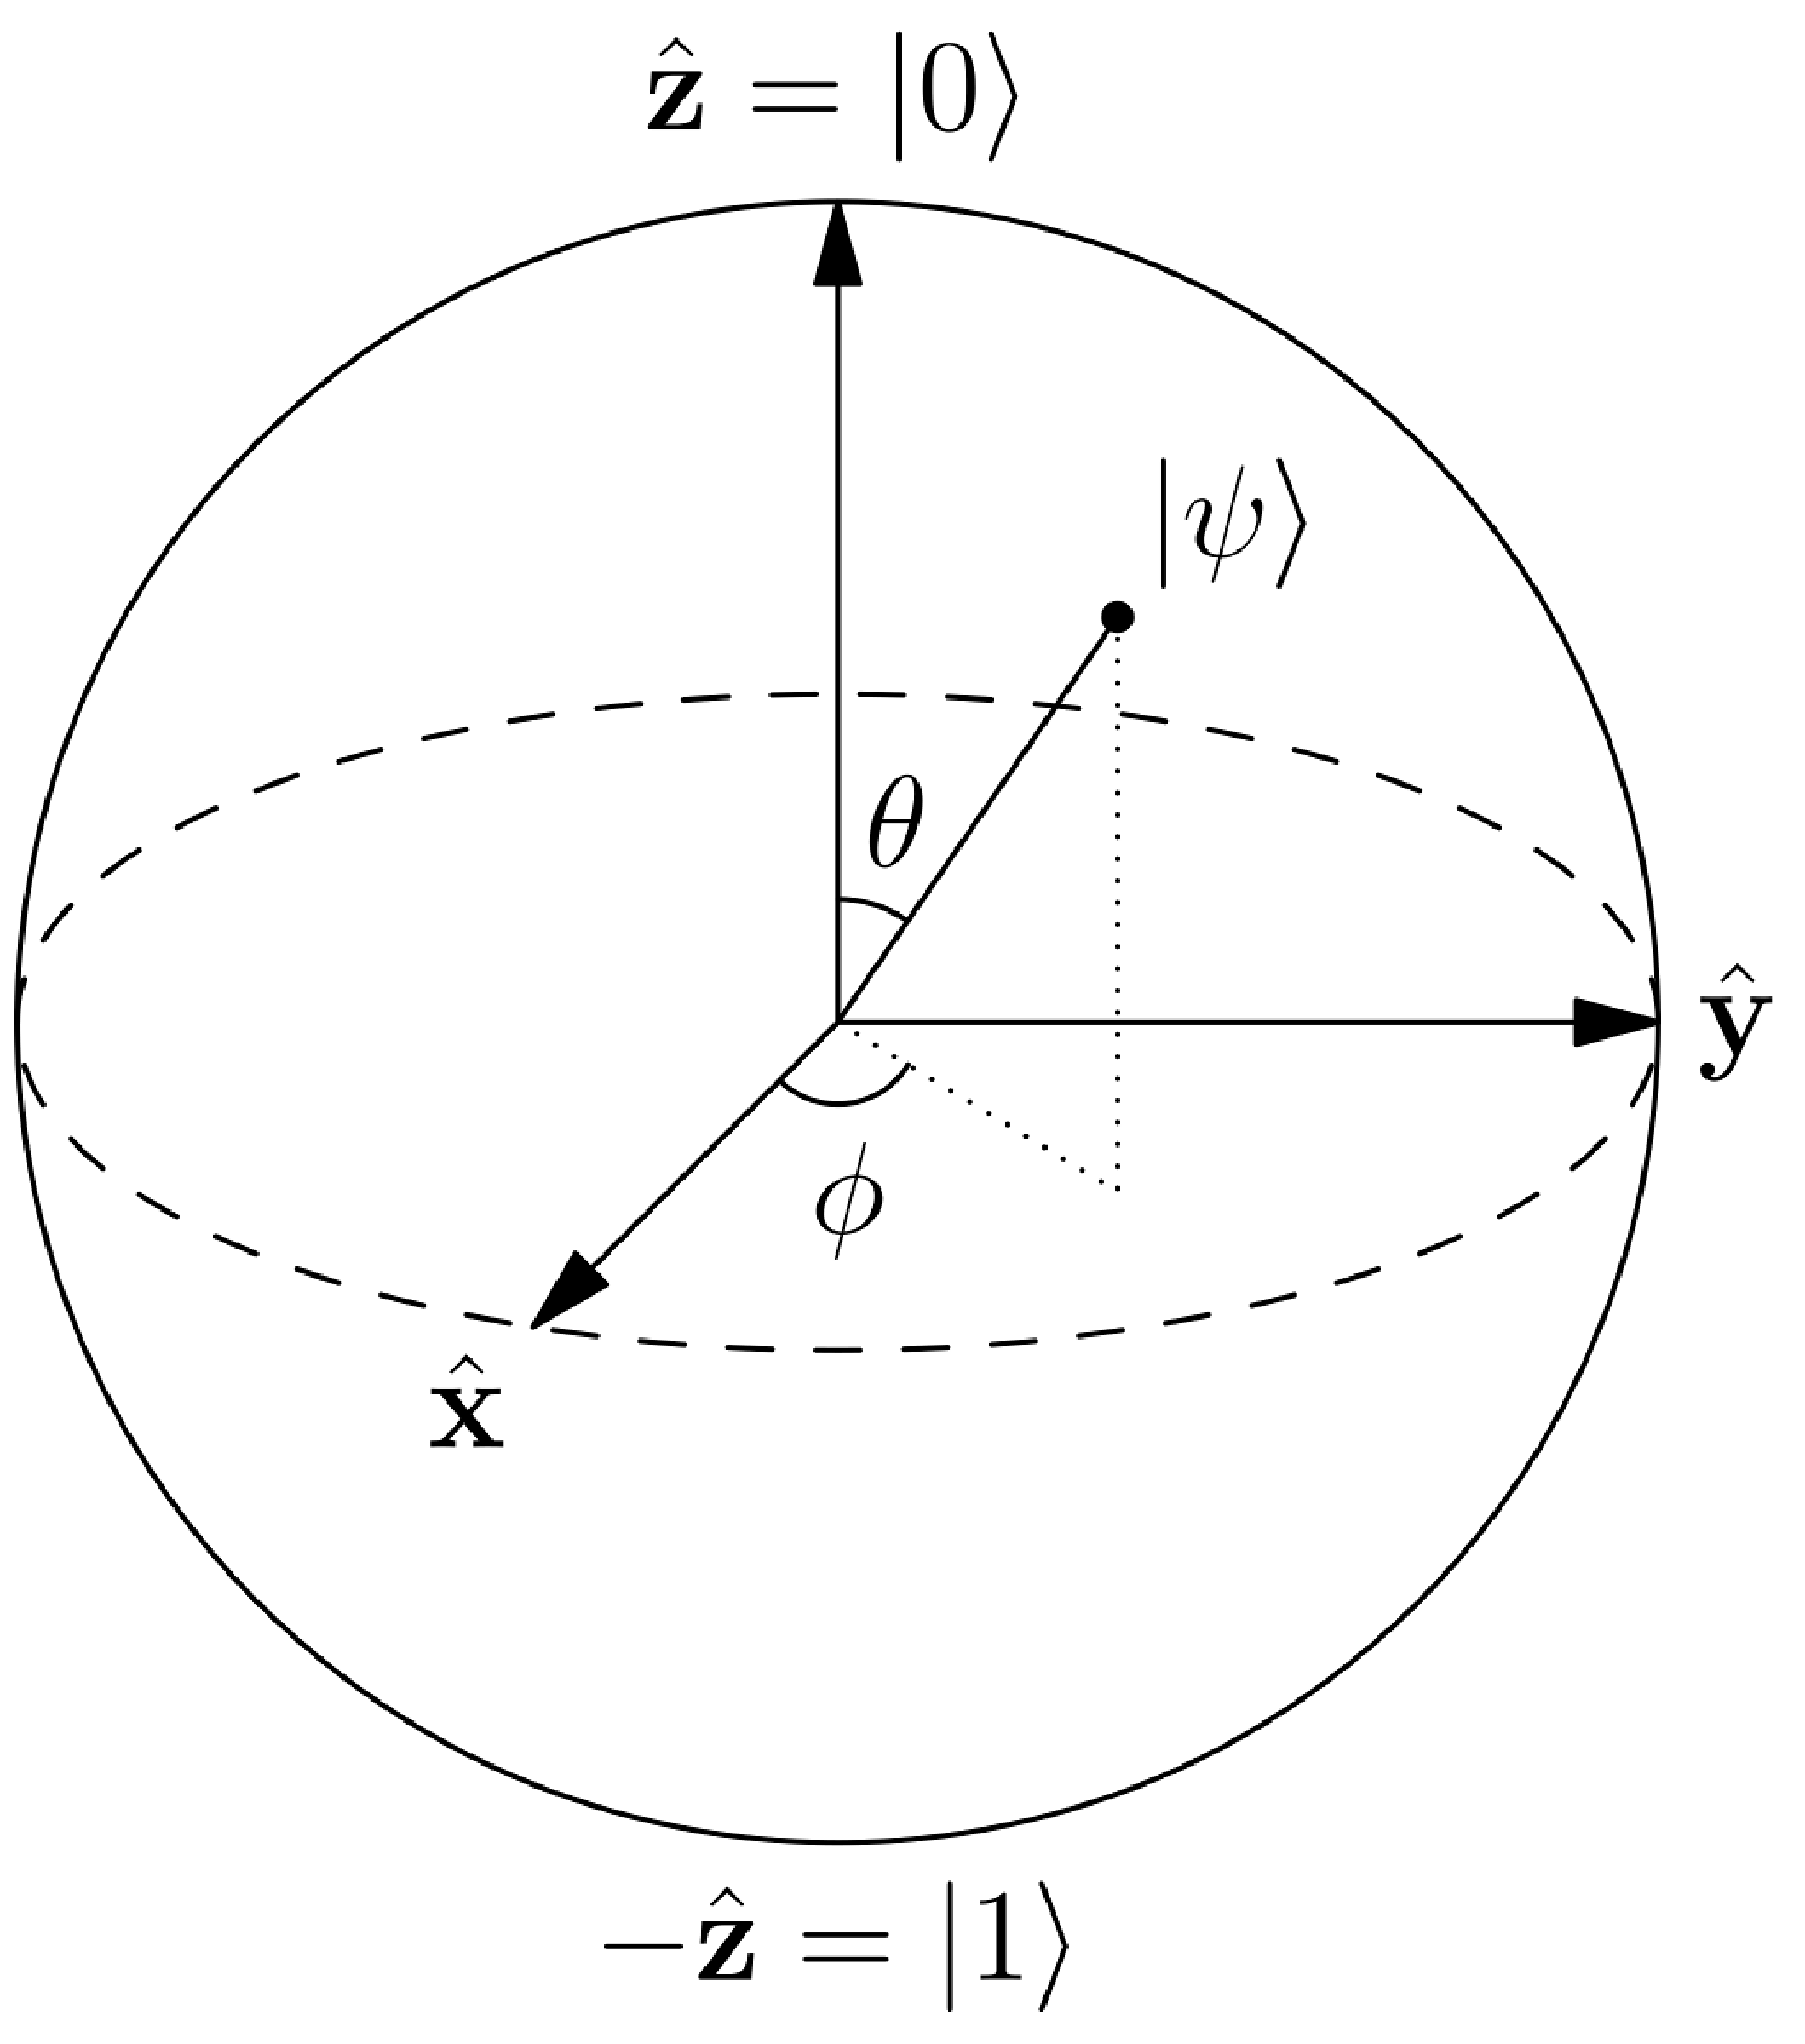
\includegraphics[scale=0.2]{images/bloch_sphere.eps}
  \caption{Bloch sphere representation of a qubit.}
  \label{fig:bloch}
\end{figure}
\par
\newpage

\subsection{Single-Qubit Quantum Operations}
Single-qubit quantum gates can be seen as rotations on the Bloch sphere. Quantum gates can be represented by matrices, which we will look at in Section~\ref{sec:matrix_notation}. These gates only have one limitation: they have to be \emph{unitary}, that is $U^\dagger U = I$, where $U^\dagger$ is the adjoint of $U$. Therefore, any $2^n \times 2^n$ unitary matrix is a valid gate which acts on $n$ qubits. Below are some notable single-qubit gates described and visualized.

\subsubsection{Pauli Gates}
 The most simple quantum gates are the \emph{Pauli} gates \emph{I}, \emph{X}, \emph{Y} and \emph{Z}. $I$ is the identity gate, which does nothing. The other gates rotate $\pi$ radians (180 degrees) around the X, Y or Z-axis. These gates are self-inverse, meaning $X = X^\dagger$.

\begin{figure}[ht]
  \begin{adjustwidth}{-2.5cm}{-2.5cm}
  \centering
  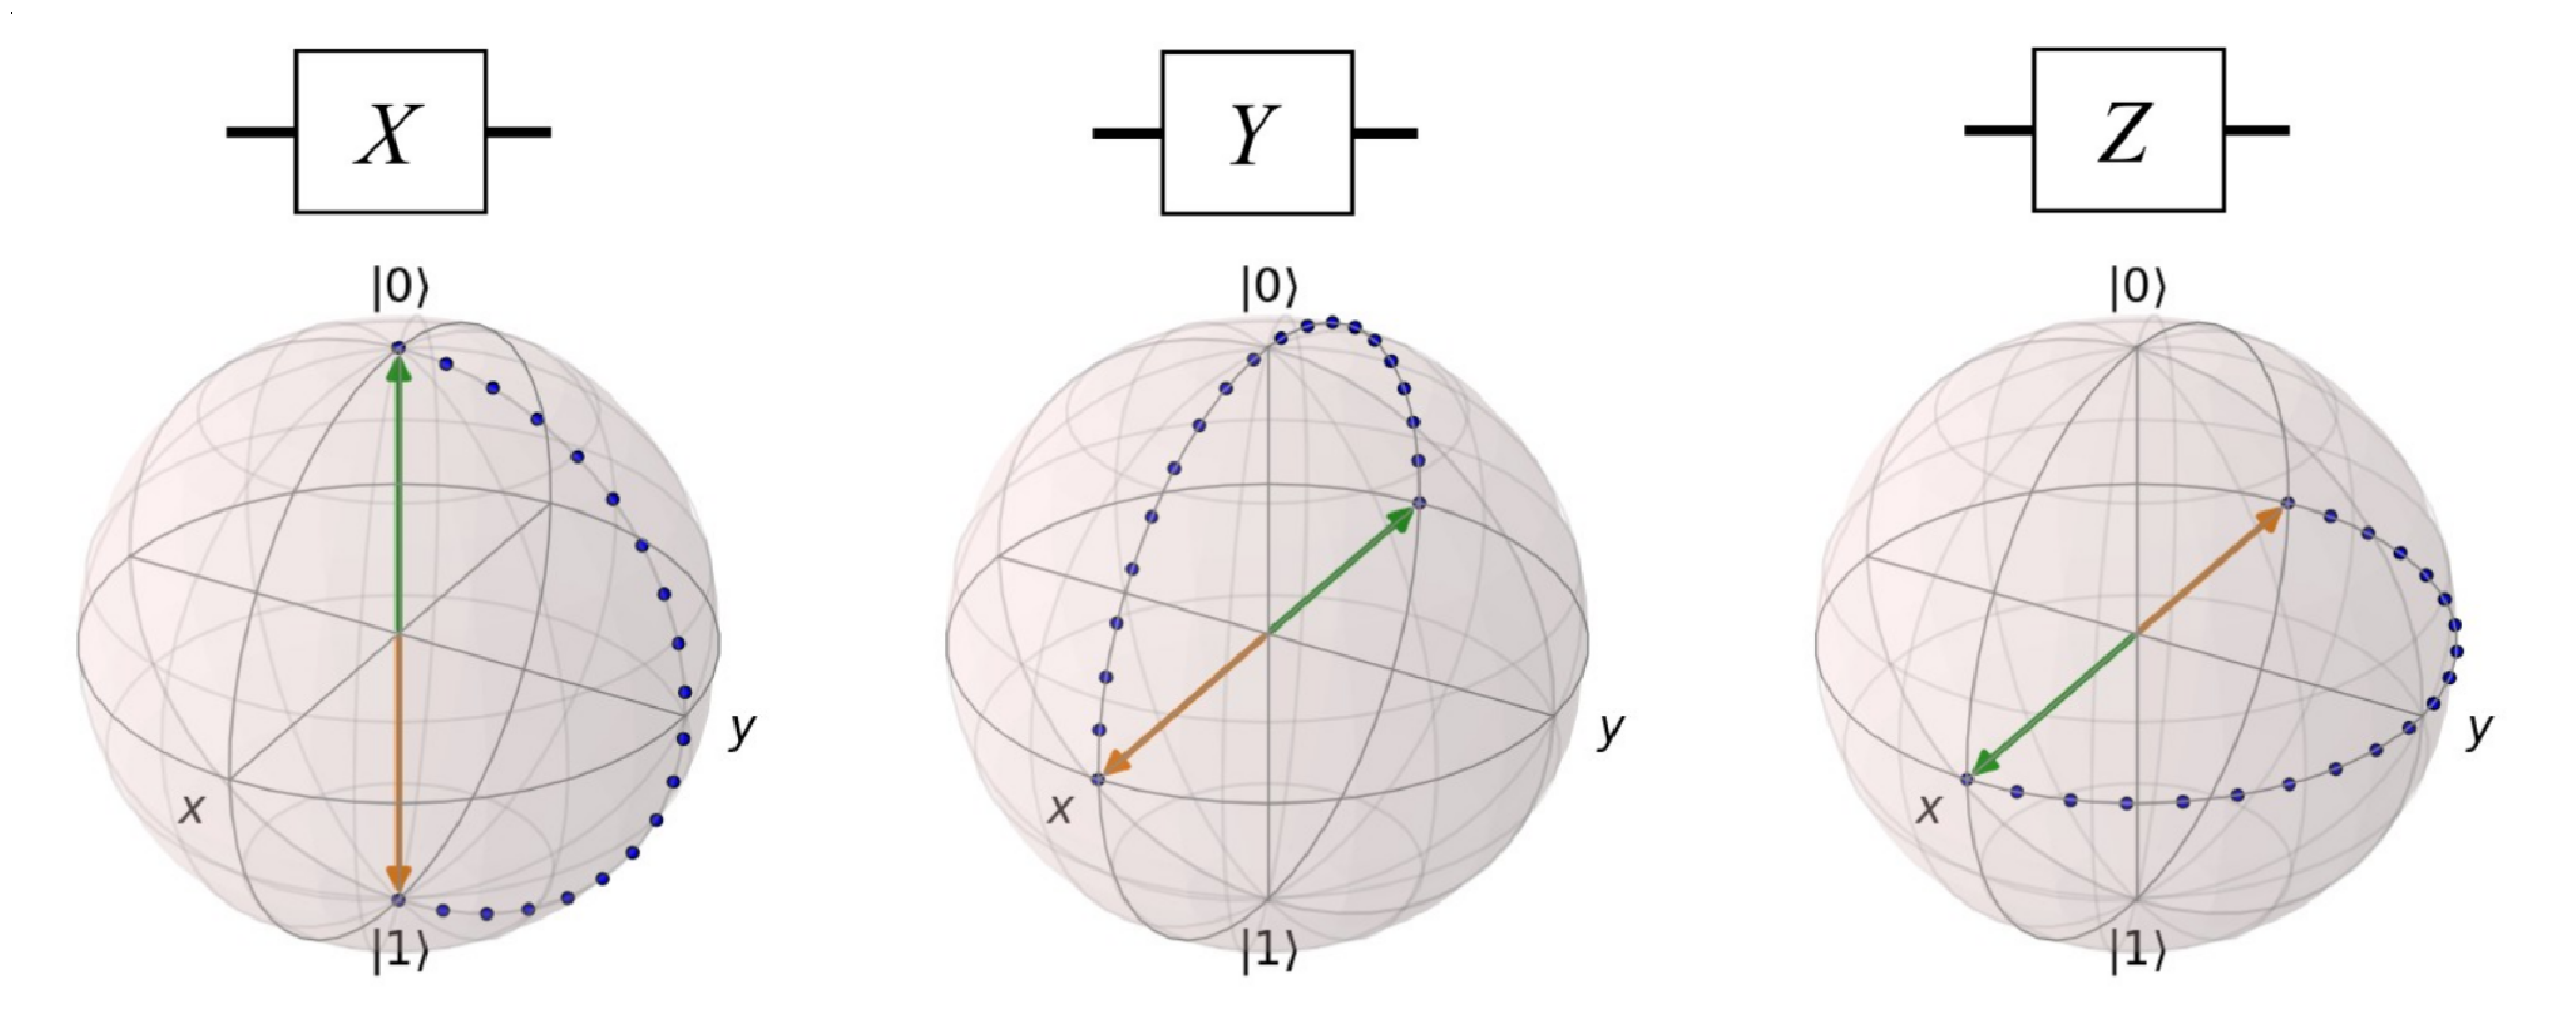
\includegraphics[scale=0.25]{images/pauli_gates.eps}
  \caption{Pauli gates $X$, $Y$ and $Z$ visualized on the Bloch sphere.}
  \end{adjustwidth}
\end{figure}

 
\subsubsection{S Gate}
The \emph{S} gate, also known as the phase (\emph{P}) gate, does a Z rotation of $\pi/2$ radians (90 degrees). It's essentially half a Pauli Z gate.

\begin{center}
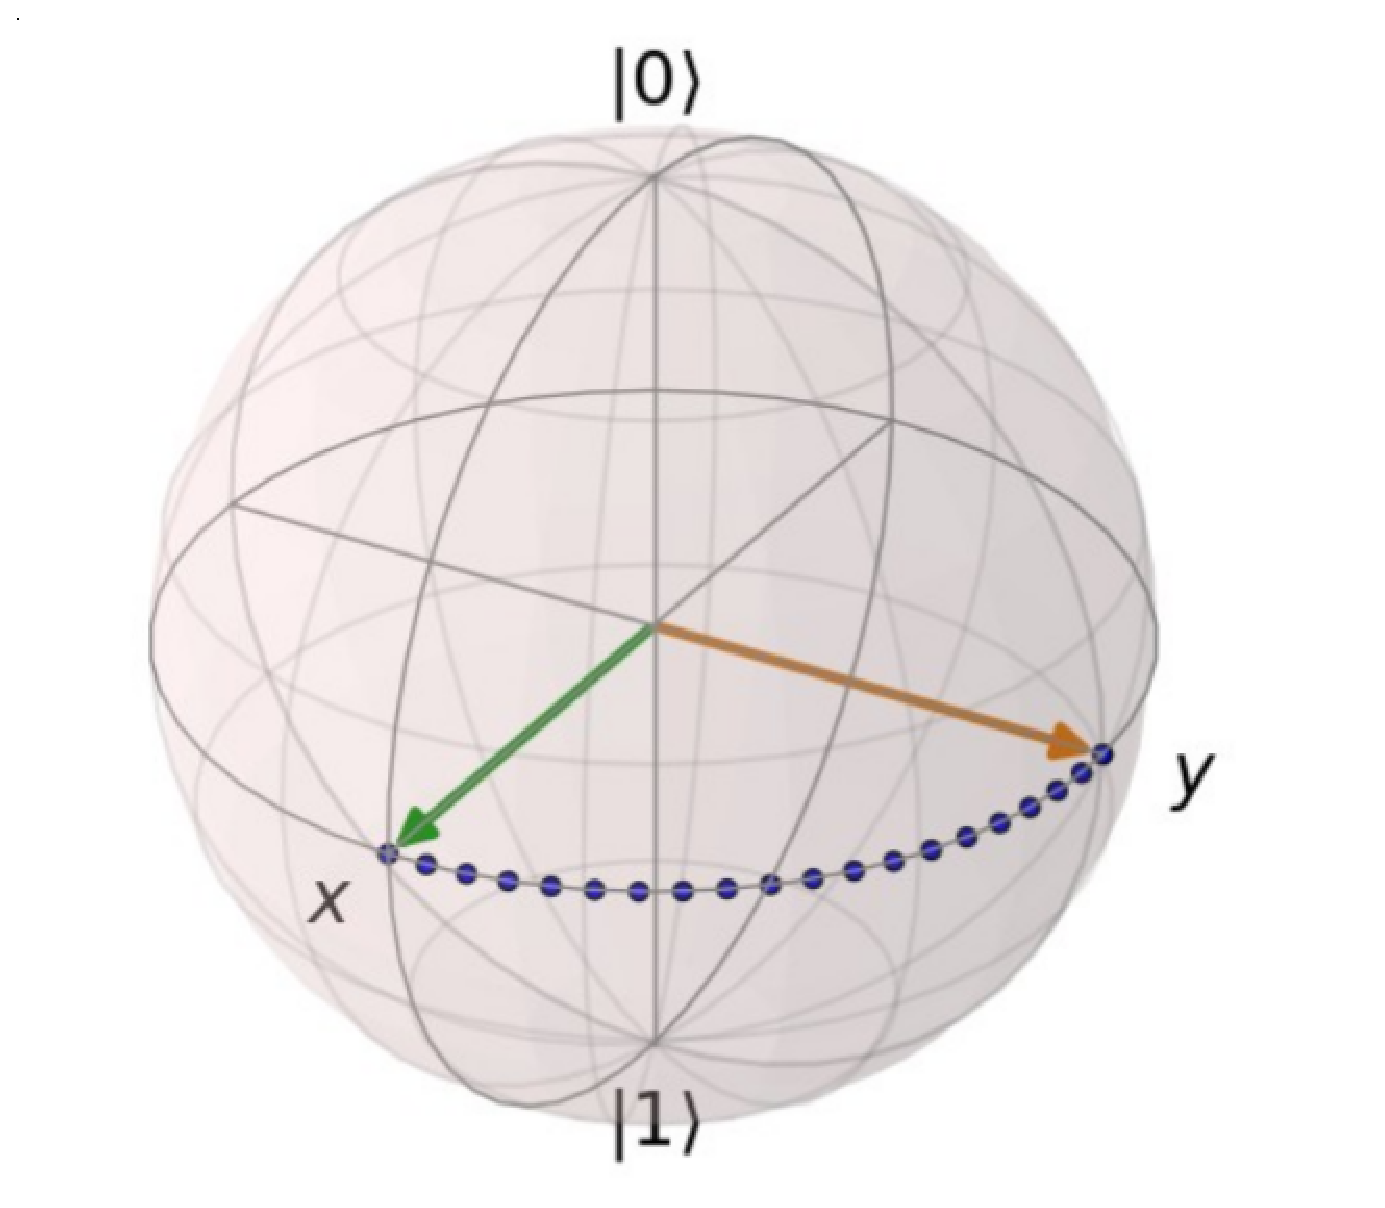
\includegraphics[scale=0.30]{images/s_gate.eps}
\end{center}

\subsubsection{Hadamard Gate}
The Hadamard gate maps the qubit-basis states $\ket{0}$ and $\ket{1}$ to superposition states with equal weight. It is the combination of two rotations, $\pi$ radians about the Z-axis followed by $\pi/2$ radians about the Y-axis. This gate is sometimes described as a ``square root of $NOT$" gate, because it turns $\ket{0}$ into $(\ket{0} + \ket{1})/\sqrt2$ (also written as $\ket{+}$), halfway between $\ket{0}$ and $\ket{1}$.

\begin{figure}[ht]
  \centering
  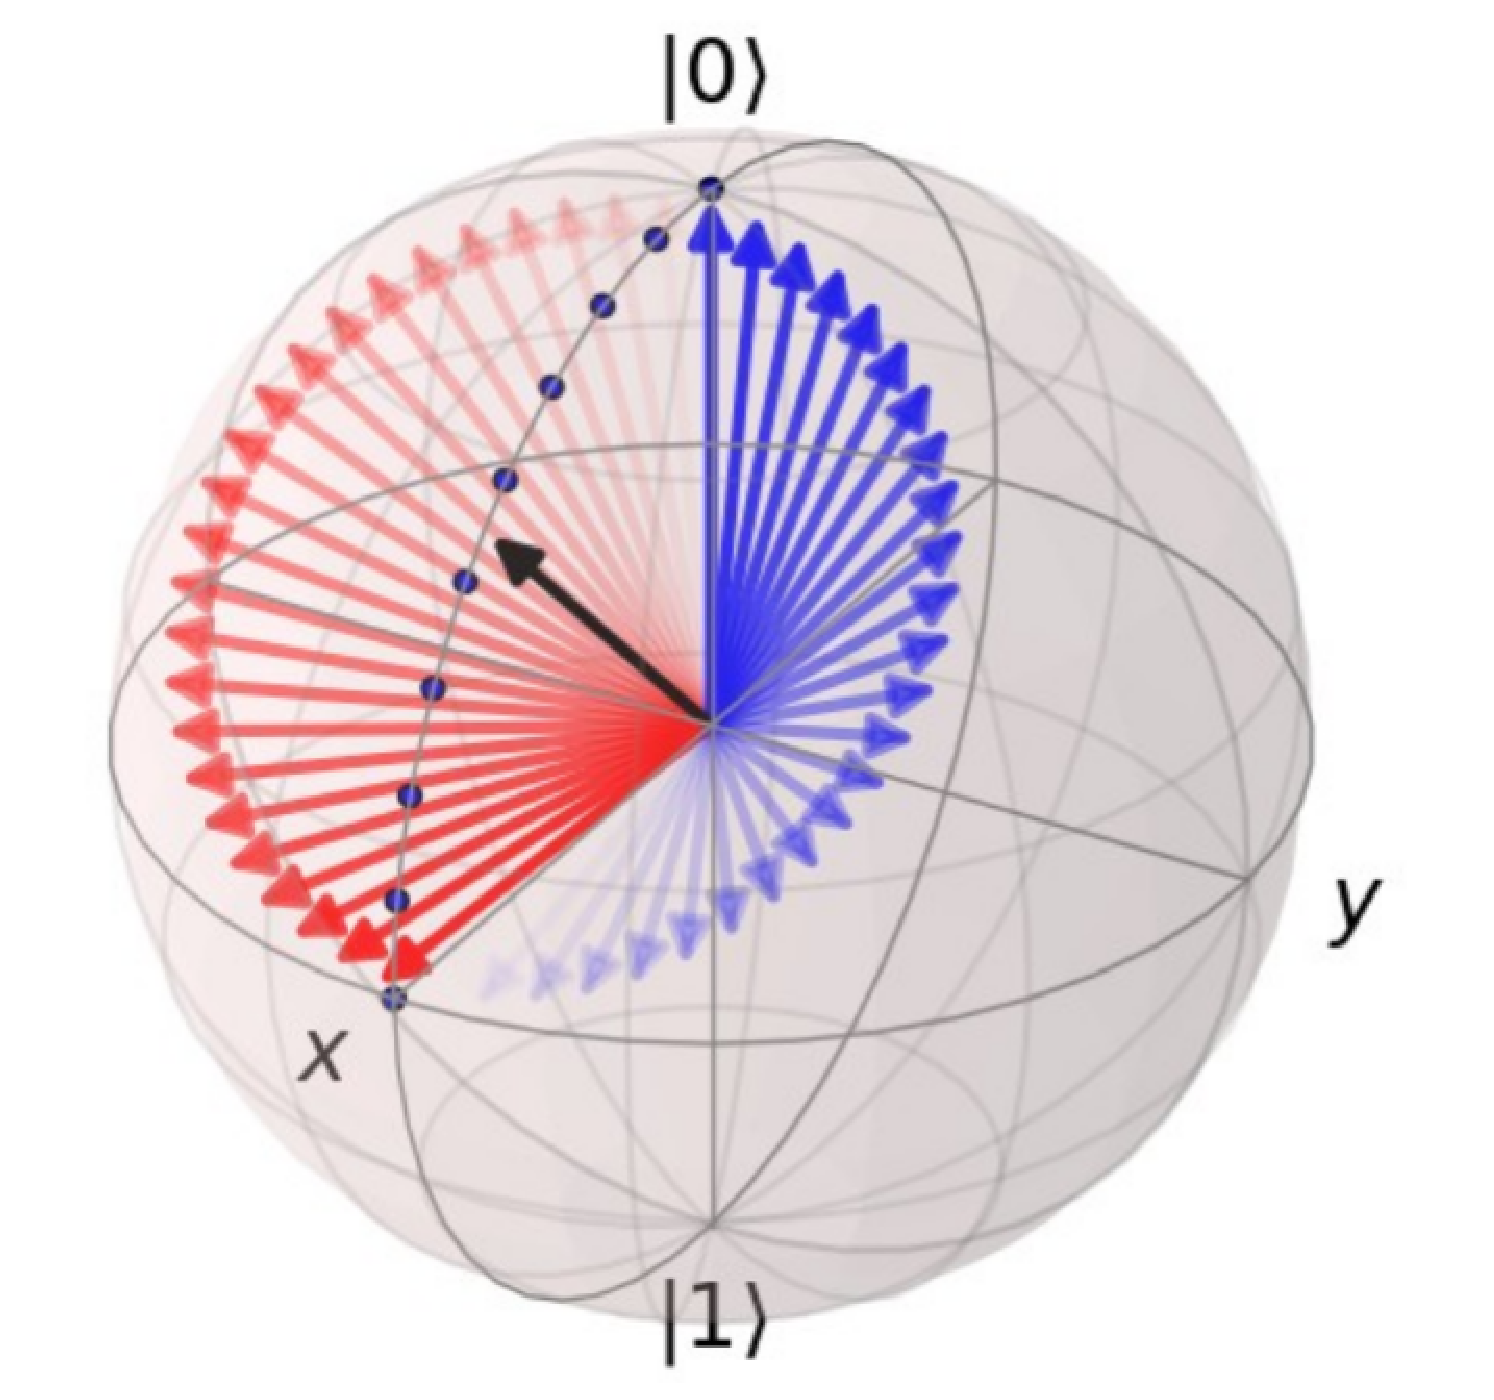
\includegraphics[scale=0.25]{images/hadamard_gate.eps}
  \caption{Hadamard gate visualized on the Bloch sphere.}
\end{figure}

\subsection{Measurement}
Measuring a qubit collapses its state. The probabilistic result of a qubit measurement can be calculated based on the probability amplitudes:
\[|\psi\rangle = \alpha\ket{0} + \beta\ket{1}\]
\[P(\ket{0}) = \left|\alpha\right|^2\]
\[P(\ket{1}) = \left|\beta\right|^2\]
Consider the following simple single-qubit circuit:

\begin{figure}[ht]
\[
  \Large{
    \Qcircuit @C=1em @R=0em {
    \push{\rule{0em}{1em}} & & \lstick{\ket{0}} & \gate{H} & \gate{Z} & \meter & \cw
    }
  }
\]
  \caption{A simple quantum circuit. The output of measuring a qubit is a classical bit, which is distinguished from a qubit by drawing a double-line wire. A visualization of this circuit on the Bloch sphere can be seen in Figure~\ref{fig:gate_rotations}.}
\end{figure}

We start with computing $H\ket{0} = \ket{+}$, followed by $Z\ket{+} = \ket{-}$. Finally we measure. We can calculate the probabilities:
\[\ket{-} = \dfrac{1}{\sqrt2} (\ket{0} - \ket{1})\]
\[P(\ket{0}) = \left|\dfrac{1}{\sqrt2}\right|^2 = \dfrac{1}{2}\]
\[P(\ket{1}) = \left|\dfrac{-1}{\sqrt2}\right|^2 = \dfrac{1}{2}\]
Giving us equal probabilities of our state being measured as $\ket{0}$ or $\ket{1}$.

\begin{figure}[ht]
  \centering
  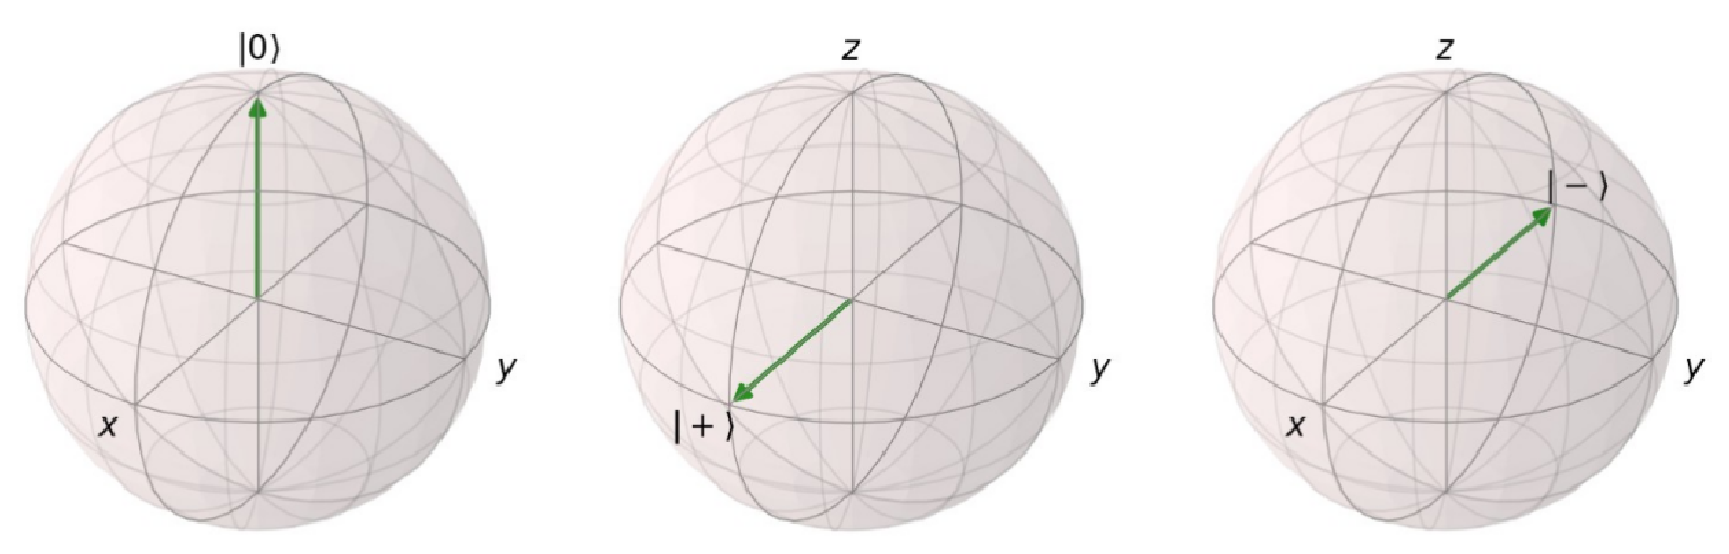
\includegraphics[scale=0.385]{images/simple_circuit.eps}
  \caption{States of our qubit throughout the circuit from left to right: \ket{0} $\rightarrow$ $H\ket{0}$ $\rightarrow$ $ZH\ket{0}.$}
  \label{fig:gate_rotations}
\end{figure}

\subsection{Matrix Notation} \label{sec:matrix_notation}
Earlier we showed that we can represent a quantum state using the following formula:
\[|\psi\rangle = \alpha\ket{0} + \beta\ket{1}\]
For computational purposes we can use vectors to represent a quantum state. We define $\ket{0}$ and $\ket{1}$ as following:
\[\ket{0} = \begin{bmatrix}1 \\ 0\end{bmatrix}\]
\[\ket{1} = \begin{bmatrix}0 \\ 1\end{bmatrix}\]
Then by filling in the formula we can represent our quantum state with a vector. This has to be a normalized vector since we are talking probabilities, where $|\alpha|^2+|\beta|^2 = 1$. In general, a qubit's state is a unit vector in a two-dimensional complex vector space.
\[|\psi\rangle = \alpha\begin{bmatrix}1\\ 0\end{bmatrix} + \beta\begin{bmatrix}0 \\ 1\end{bmatrix} =
\begin{bmatrix}\alpha \\ \beta\end{bmatrix}\]
The single-qubit gates can then be represented by $2 \times 2$ unitary matrices:
\setlength\multicolsep{0pt}
\begin{multicols}{3}
  \[
    I =
    \begin{bmatrix}
    1 & 0 \\
    0 & 1 
    \end{bmatrix}
  \]
  \vfill
  \[
    X =
    \begin{bmatrix}
    0 & 1 \\
    1 & 0 
    \end{bmatrix}
  \]
  \vfill
  \[
    Y =
    \begin{bmatrix}
    0 & -i \\
    i & \phantom{-}0
    \end{bmatrix}
  \]
\end{multicols}

\begin{multicols}{3}
  \[
    Z =
    \begin{bmatrix}
    1 & \phantom{-}0 \\
    0 & -1
    \end{bmatrix}
  \]
  \vfill
  \[
    H = \dfrac{1}{\sqrt2}
    \begin{bmatrix}
    1 & \phantom{-}1 \\
    1 & -1
    \end{bmatrix}
  \]
  \vfill
  \[
    S =
    \begin{bmatrix}
    1 & 0 \\
    0 & i
    \end{bmatrix}
  \]
\end{multicols}
\bigskip
\noindent
Then a computation like $X\ket{0}$ can be calculated by matrix vector multiplication:
\[
X\ket{0} = 
\begin{bmatrix}
0 & 1 \\
1 & 0
\end{bmatrix}
\begin{bmatrix}1 \\ 0\end{bmatrix} =
\begin{bmatrix}0 \\ 1\end{bmatrix}
\]
And we find that $X\ket{0} = \ket{1}$. Or, more general:
\[
X\begin{bmatrix}\alpha \\ \beta\end{bmatrix} = \begin{bmatrix}\beta \\ \alpha\end{bmatrix}
\]
\end{document}
